\documentclass[a4paper]{article}

\title{PH2255 Course:\\
Introduction to Statistical Methods\\Exercise 3}
\author{Thomas Bass}
\date{29 January 2021}

% LaTeX preambule: loading relevant packages, configuring Python listings
\usepackage{graphicx}
\usepackage{amsmath}
\usepackage{color}
\usepackage{listings}
\usepackage{hyperref}
\usepackage{bm}

\definecolor{dkgreen}{rgb}{0,0.6,0}
\definecolor{gray}{rgb}{0.5,0.5,0.5}
\definecolor{mauve}{rgb}{0.58,0,0.82}

% Settings for colour-coding and formatting Python code:
\lstset{
  language=Python,                % the language of the code
  basicstyle=\footnotesize,           % the size of the fonts that are used for the code
  numbers=left,                   % where to put the line-numbers
  numberstyle=\tiny\color{gray},  % the style that is used for the line-numbers
  stepnumber=5,                   % the step between two line-numbers. If it's 1, each line
                                  % will be numbered
  numbersep=5pt,                  % how far the line-numbers are from the code
  backgroundcolor=\color{white},      % choose the background color. You must add \usepackage{color}
  showspaces=false,               % show spaces adding particular underscores
  showstringspaces=false,         % underline spaces within strings
  showtabs=false,                 % show tabs within strings adding particular underscores
  frame=single,                   % adds a frame around the code
  rulecolor=\color{black},        % if not set, the frame-color may be changed on line-breaks within not-black text (e.g. commens (green here))
  tabsize=2,                      % sets default tabsize to 2 spaces
  captionpos=b,                   % sets the caption-position to bottom
  breaklines=true,                % sets automatic line breaking
  breakatwhitespace=false,        % sets if automatic breaks should only happen at whitespace
  title=\lstname,                   % show the filename of files included with \lstinputlisting;
                                  % also try caption instead of title
  keywordstyle=\color{blue},          % keyword style
  commentstyle=\color{dkgreen},       % comment style
  stringstyle=\color{mauve},         % string literal style
  escapeinside={\%*}{*)},            % if you want to add LaTeX within your code
  morekeywords={*,...}               % if you want to add more keywords to the set
}

\begin{document}
\maketitle

\begin{abstract}
Exercise 3 of PH2255 introduces us to another real-world historical application of the methods we have learned. By applying the $\chi^2_\text{min}$ method to one of Ptolemy's experiments - investigating the refraction of light through an air-water medium - we can compare it to a common hypothesis at the time, the hypothesis Ptolemy used, and one first discovered by Ibn Sahl in the 10th Century (later re-discovered by Snell in 1621).
\end{abstract}

First, we start by ingesting the data given in the lab script, using Numpt's \lstinline$np.array$ for easy data manipulation later on, especially with trig functions. The errors for each measurement were not recorded, so we assume $\sigma = \frac12\deg$ for $\theta_r$, as Ptolemy's measurements were all given in half-degree increments. We do not use errors on $\theta_i$, as such errors would be absorbed into $\theta_r$
\begin{lstlisting}
t_i = np.array([10.0, 20.0, 30.0, 40.0, 50.0, 60.0, 70.0, 80.0])
t_r = np.array([8.0,  15.5, 22.5, 29.0, 35.0, 40.5, 45.5, 50.0])
sig = np.array([0.5,  0.5,  0.5,  0.5,  0.5,  0.5,  0.5,  0.5])
\end{lstlisting}

Next, we set up the two hypotheses used in part {\it a}, the first being the commonly accepted hypothesis at the time, and the second being Ptolemy's new hypothesis:
\begin{equation}
\theta_r=\alpha\theta_i
\end{equation}
\begin{equation}
\theta_r=\alpha\theta_i - \beta\theta_i^2
\end{equation}
Defining these in Python, we get the following:
\begin{lstlisting}
def h1(t_i, *vars):
    a, = vars
    return a*t_i

def h2(t_i, *vars):
    a, b = vars
    return a*t_i - b*t_i**2
\end{lstlisting}
We use the same techniques as previous weeks to fit these functions to the data points: by using SciPy's \lstinline$curve_fit$ function, we get the fit's parameters and covariances. From these, we can plot the fits along with one standard deviation above and below the fit, resulting in the following plots: 

\begin{figure}[h!]
\centerline{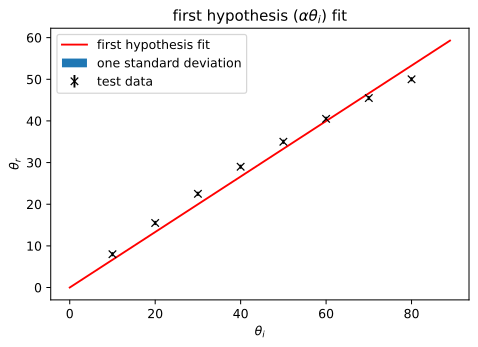
\includegraphics[scale=0.7]{fit1.png}}
\caption{First hypothesis fit, showing the data points, fit curve, and one standard deviation above and below the fit.}
\label{fig:fit1}
\end{figure}

\begin{figure}[h!]
\centerline{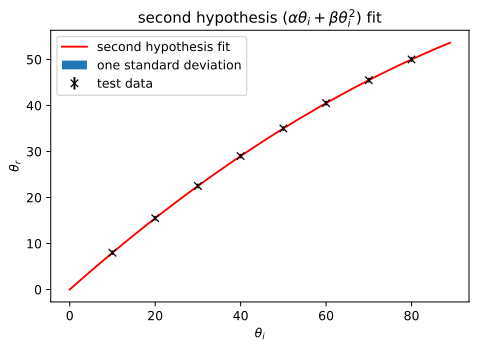
\includegraphics[scale=0.7]{fit2.png}}
\caption{Second hypothesis fit, showing the data points, fit curve, and one standard deviation above and below the fit.}
\label{fig:fit2}
\end{figure}

The parameters for these fits are listed below in Table \ref{tab:params1}

\begin{table}[h!]
\centering
\begin{tabular}{ccc}
\hline
Hypothesis Fit & $\alpha$ & $\beta$\\ \hline
1 & 0.666 & n/a \\
2 & 0.825 & 0.0025 \\
\end{tabular}
\caption{\label{tab:params1}Parameters for the fitted functions of the first two hypotheses.}
\end{table}

To quantify the {\it "goodness-of-fit"} for these, we again employ the $\chi^2_\text{min}$ value, and the associated {\it p-value}. To obtain these values, we use the following Python functions, employing SciPy's \lstinline$stats.chi2$ function:

\begin{lstlisting}
chi_sq_min = sum(((d - f1(h, *theta_hat))/sig)**2)
ndof = len(h)-len(p0)
p_val = scipy.stats.chi2.sf(chi_sq_min, df=ndof)
\end{lstlisting}

From this, we generate the following $\chi^2_\text{min}$  and p-values:

\begin{table}[h!]
\centering
\begin{tabular}{ccc}
\hline
Hypothesis Fit & $\chi^2_\text{min}$/NDoF & {\it p-value}\\ \hline
1 & $19.24$ & $6.71\times10^{-26}$ \\
2 & $0.0$ & $1.0$ \\
\end{tabular}
\caption{\label{tab:chi1}Parameters for the fitted functions of the first two hypotheses.}
\end{table}

The results of $\chi^2_\text{min}$=0 for the second hypothesis is extremely unusual - it indicates that the fit matches the data {\it far better} than expected, and does not have the expected standard deviation given by our choice of errors. This indicates to us that some of the data may have been inferred and not measured - perhaps the angles below 45 degrees were merely doubled by Ptolemy and recorded as the angles above 45 degrees.

To analyse this further, and to use a third hypothesis, we use the following equation first discovered by Ibn Sahl in the 10th century, later rediscovered by Snell in 1621, and commonly known as Snell's Law:

\begin{equation}
\theta_r=\sin^{-1}\left(\frac{\sin\theta_i}r\right)
\end{equation}

We use the exact same analysis for this third hypothesis as the first two: using the minimisation of residuals method offered by \lstinline$curve_fit$, and calculating the $\chi^2_\text{min}$ and p-value for the fit. Plotting the fitted parameters gives us the following figure:

\begin{figure}[hb!]
\centerline{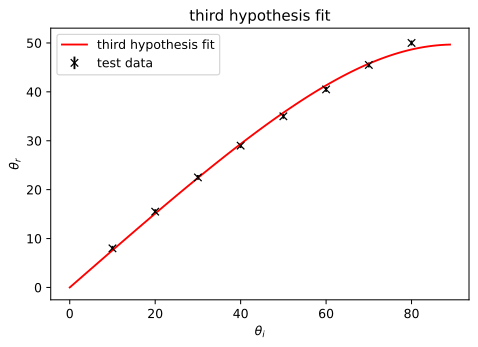
\includegraphics[scale=0.5]{fit3.png}}
\caption{Third hypothesis fit, showing the data points, fit curve, and one standard deviation above and below the fit.}
\label{fig:fit3}
\end{figure}

With the calculated parameter $r=1.31$  

By applying the $\chi^2_\text{min}$ method, we find $\chi^2_\text{min}=2.00$ and $\text{\it{p-value}}=0.05$. These values are far more within the realm of expectation for our error bars, and methodology. From looking at the plot, we can see that the final data point is by far the outlier: from this we could reject the hypothesis, but the rest of the data points hold well. Instead, we could challenge the assumption of $\sigma=\frac12\deg$, and instead investigate the results with a larger error width.

\begin{appendix}
\section{Python Code}\label{sec:python}
\lstinputlisting[language=Python,frame=single]{py.py}

\begin{verbatim}
---Hypothesis 1---
Chi-sq-min/NDoF:	19.235294117647054
p-value:		6.711003202955456e-26
---Hypothesis 2---
Chi-sq-min/NDoF:	0.0
p-value:		1.0
---Hypothesis 3---
Chi-sq-min/NDoF:	2.0003105594271977
p-value:		0.05114270171746438
\end{verbatim}

\begin{verbatim}
Hypothesis 1:	 a = 0.6661764705875071
Hypothesis 2:	 a = 0.825	b = 0.0024999999999999996
Hypothesis 3:	 r = 1.3116118503798777
\end{verbatim}

\end{appendix}

\end{document}
